% Propositions de remplacement pour la Figure 3 (P1-2).
% Document autonome : ne modifie pas main_position.tex.
% Compilation : pdflatex fig3_alternatives.tex
\documentclass[10pt]{article}
\usepackage[margin=1.6cm,a4paper,landscape]{geometry}
\usepackage[T1]{fontenc}
\usepackage{lmodern}
\usepackage{booktabs}
\usepackage{array}
\usepackage{xcolor}
\usepackage{tikz}
\usepackage{amssymb}
\usetikzlibrary{arrows.meta,positioning,calc,shapes.geometric}
\usepackage{caption}
\captionsetup{font=small,labelfont=bf}

\definecolor{clrH}{RGB}{155,18,18}
\definecolor{clrLD}{RGB}{22,98,48}
\definecolor{clrB}{RGB}{22,52,125}
\definecolor{clrO}{RGB}{170,91,24}
\definecolor{clrP}{RGB}{92,61,145}
\definecolor{clrG}{RGB}{80,80,80}

\newcommand{\yes}{\textcolor{clrLD}{$\blacksquare$}}
\newcommand{\hf}{\textcolor{clrO}{$\square$}}
\newcommand{\no}{\textcolor{clrG!45}{$\cdot$}}

\begin{document}
\pagestyle{empty}

\begin{center}
{\Large\bfseries Figure 3 --- trois propositions de remplacement}\\[2pt]
{\small Donn\'ees : les 41 ressources du mapping, Tableaux B.1--B.3. Aucune valeur invent\'ee.}
\end{center}

\vspace{4pt}
\noindent\rule{\linewidth}{0.4pt}

\section*{Ce que disent les donn\'ees (v\'erifi\'e sur les 41 lignes)}
\noindent
\begin{tabular}{@{}lll@{}}
\toprule
\textbf{Champ} & \textbf{Valeurs observ\'ees sur 41 ressources} & \textbf{Cons\'equence pour la figure}\\
\midrule
Task oracle $O$ & 15 types explicites ; 6 \emph{none identifiable} ; 15 \emph{mixed} & varie r\'eellement : m\'erite une colonne\\
Permission scope $\Gamma$ & 22 \emph{inferred empty} ; 10 \emph{not separately repr.} ; & \textbf{0 ressource d\'eclare $\Gamma$ explicitement}\\
                          & 8 \emph{implicit frame} ; 1 \emph{partial} & \\
Required status marking $\mu$ & 26 \emph{not scored} ; 15 \emph{not separated} & \textbf{0/41. Colonne enti\`erement vide}\\
Style-marking control & 34 \emph{not controlled} ; 6 \emph{n.c. or N/A} ; & \textbf{1/41 seulement} : s\'epare 1 ressource de 40\\
                      & 1 \emph{scored, not claim-controlled} (WritingBench) & \\
\bottomrule
\end{tabular}

\vspace{6pt}
\noindent\textbf{Diagnostic de la figure actuelle.} L'axe vertical de la Figure~3 encode le traitement du
style-marking, c'est-\`a-dire une variable dont \textbf{une seule ressource sur 41} prend une valeur non
par d\'efaut. Un axe entier est donc consacr\'e \`a s\'eparer WritingBench des quarante autres, tandis que le
r\'esultat annonc\'e --- \emph{aucune ressource ne repr\'esente s\'epar\'ement $O$, $\Gamma$ et $\mu$} --- n'appara\^it
pas dans la figure et doit \^etre affirm\'e en l\'egende. Les trois propositions ci-dessous font l'inverse :
elles montrent le r\'esultat et rel\`eguent le style au rang de colonne parmi d'autres.

\clearpage

\section*{Proposition A --- Matrice de couverture par profil \quad {\normalfont\itshape (recommand\'ee)}}

\vspace{2pt}
\begin{center}
\resizebox{0.97\linewidth}{!}{%
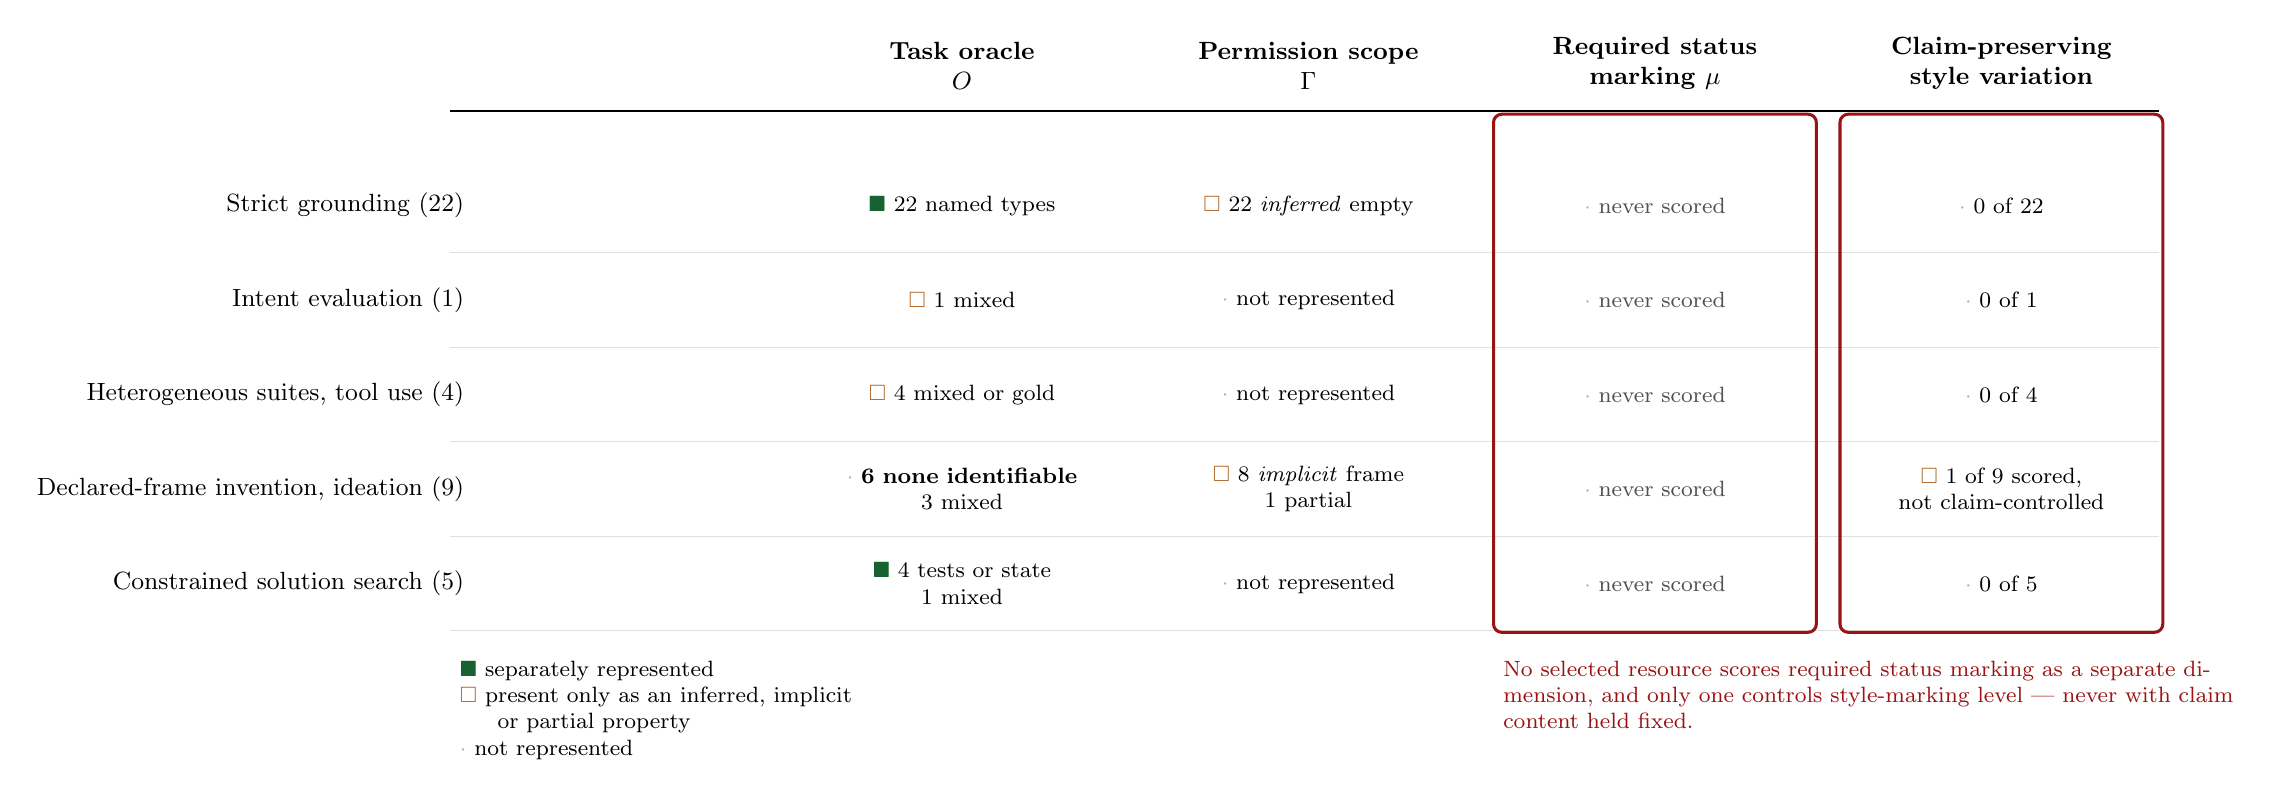
\begin{tikzpicture}[x=1cm,y=1cm,font=\small]
  \def\colA{0} \def\colB{4.4} \def\colC{8.8} \def\colD{13.2}
  \def\lx{-6.2}

  \node[anchor=south,align=center,font=\small\bfseries] at (\colA,0.35) {Task oracle\\$O$};
  \node[anchor=south,align=center,font=\small\bfseries] at (\colB,0.35) {Permission scope\\$\Gamma$};
  \node[anchor=south,align=center,font=\small\bfseries] at (\colC,0.35) {Required status\\marking $\mu$};
  \node[anchor=south,align=center,font=\small\bfseries] at (\colD,0.35) {Claim-preserving\\style variation};
  \draw[semithick] (\lx-0.3,0.2) -- (\colD+2.0,0.2);

  \foreach \y/\prof in {%
    -1.0/{Strict grounding (22)},
    -2.2/{Intent evaluation (1)},
    -3.4/{Heterogeneous suites, tool use (4)},
    -4.6/{Declared-frame invention, ideation (9)},
    -5.8/{Constrained solution search (5)}}{
      \node[anchor=east,align=right,font=\small] at (\lx,\y) {\prof};
      \draw[draw=black!12] (\lx-0.3,\y-0.6) -- (\colD+2.0,\y-0.6);
  }

  % --- O ---
  \node[align=center,font=\footnotesize,text width=3.9cm] at (\colA,-1.0) {\yes\ 22 named types};
  \node[align=center,font=\footnotesize,text width=3.9cm] at (\colA,-2.2) {\hf\ 1 mixed};
  \node[align=center,font=\footnotesize,text width=3.9cm] at (\colA,-3.4) {\hf\ 4 mixed or gold};
  \node[align=center,font=\footnotesize,text width=3.9cm] at (\colA,-4.6) {\no\ \textbf{6 none identifiable}\\3 mixed};
  \node[align=center,font=\footnotesize,text width=3.9cm] at (\colA,-5.8) {\yes\ 4 tests or state\\1 mixed};

  % --- Gamma ---
  \node[align=center,font=\footnotesize,text width=3.9cm] at (\colB,-1.0) {\hf\ 22 \emph{inferred} empty};
  \node[align=center,font=\footnotesize,text width=3.9cm] at (\colB,-2.2) {\no\ not represented};
  \node[align=center,font=\footnotesize,text width=3.9cm] at (\colB,-3.4) {\no\ not represented};
  \node[align=center,font=\footnotesize,text width=3.9cm] at (\colB,-4.6) {\hf\ 8 \emph{implicit} frame\\1 partial};
  \node[align=center,font=\footnotesize,text width=3.9cm] at (\colB,-5.8) {\no\ not represented};

  % --- mu : entirely empty ---
  \foreach \y in {-1.0,-2.2,-3.4,-4.6,-5.8}{
    \node[align=center,font=\footnotesize,text width=3.9cm] at (\colC,\y)
      {\no\ \textcolor{clrG}{never scored}};}
  \draw[clrH,line width=1.1pt,rounded corners=3pt]
     (\colC-2.05,-6.42) rectangle (\colC+2.05,0.16);

  % --- style ---
  \node[align=center,font=\footnotesize,text width=3.9cm] at (\colD,-1.0) {\no\ 0 of 22};
  \node[align=center,font=\footnotesize,text width=3.9cm] at (\colD,-2.2) {\no\ 0 of 1};
  \node[align=center,font=\footnotesize,text width=3.9cm] at (\colD,-3.4) {\no\ 0 of 4};
  \node[align=center,font=\footnotesize,text width=3.9cm] at (\colD,-4.6) {\hf\ 1 of 9 scored,\\not claim-controlled};
  \node[align=center,font=\footnotesize,text width=3.9cm] at (\colD,-5.8) {\no\ 0 of 5};
  \draw[clrH,line width=1.1pt,rounded corners=3pt]
     (\colD-2.05,-6.42) rectangle (\colD+2.05,0.16);

  \node[anchor=north west,align=left,font=\footnotesize,text=clrH,text width=9.5cm]
    at (\colC-2.05,-6.66)
    {No selected resource scores required status marking as a separate dimension,
     and only one controls style-marking level --- never with claim content held fixed.};

  \node[anchor=north west,align=left,font=\footnotesize] at (\lx-0.3,-6.66)
    {\yes\ separately represented\\
     \hf\ present only as an inferred, implicit\\ \hspace*{1.6em}or partial property\\
     \no\ not represented};
\end{tikzpicture}}
\end{center}

\vspace{2pt}
\noindent\textbf{Pourquoi elle fonctionne.}
(i) Le r\'esultat principal du papier --- l'absence de la combinaison compl\`ete --- devient
\emph{visible} : deux colonnes sont vides, ce que la l\'egende n'a plus \`a affirmer.
(ii) La grille est cat\'egorielle par construction : aucune distance n'est sugg\'er\'ee, donc les
quatre phrases d'avertissement de la l\'egende actuelle et l'encadr\'e \emph{Reading guide} disparaissent.
(iii) La distinction \emph{d\'eclar\'e} / \emph{inf\'er\'e} (\yes\ vs \hf) porte un point que la figure actuelle ne
peut pas montrer : $\Gamma$ n'est jamais absent au sens strict, il est toujours devin\'e par le codeur.
(iv) Le style redevient une colonne parmi quatre, ce qui corrige la sur-repr\'esentation
signal\'ee en revue.

\medskip
\noindent\textbf{Co\^ut.} Une demi-page en pleine largeur. Remplace la figure actuelle sans perte
d'information : les num\'eros de ressources restent dans les Tableaux B.1--B.3, auxquels la l\'egende renvoie.

\clearpage

\section*{Proposition B --- Grille ressource par ressource}

\vspace{-2pt}
\begin{center}
\resizebox{\linewidth}{!}{%
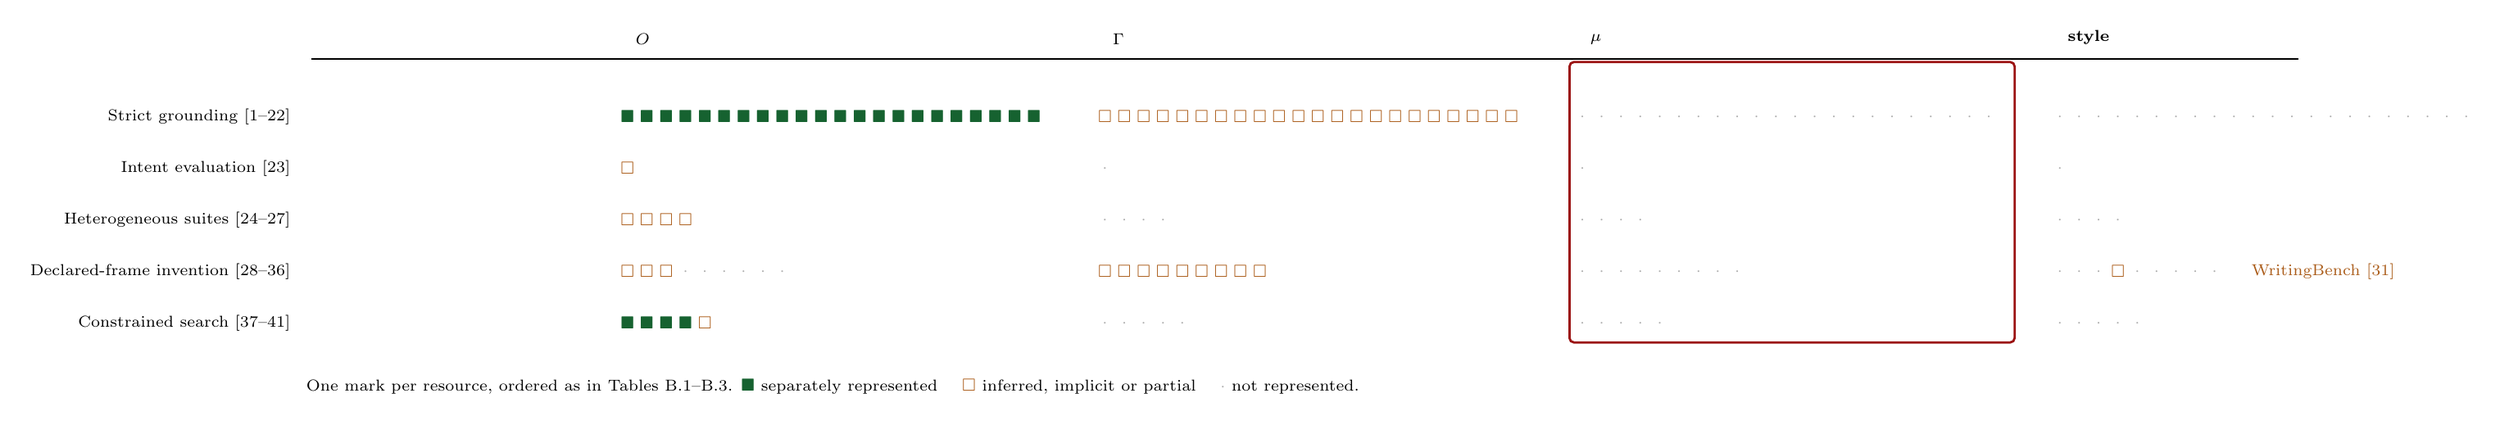
\begin{tikzpicture}[x=1cm,y=1cm,font=\scriptsize]
  \def\dx{0.30}
  \node[anchor=south west,font=\scriptsize\bfseries] at (0,0.25) {$O$};
  \node[anchor=south west,font=\scriptsize\bfseries] at (7.4,0.25) {$\Gamma$};
  \node[anchor=south west,font=\scriptsize\bfseries] at (14.8,0.25) {$\mu$};
  \node[anchor=south west,font=\scriptsize\bfseries] at (22.2,0.25) {style};
  \draw[semithick] (-4.9,0.15) -- (25.9,0.15);

  % rows: profile bands
  \foreach \y/\lab in {%
    -0.75/{Strict grounding [1--22]},
    -1.55/{Intent evaluation [23]},
    -2.35/{Heterogeneous suites [24--27]},
    -3.15/{Declared-frame invention [28--36]},
    -3.95/{Constrained search [37--41]}}{
      \node[anchor=east,font=\scriptsize] at (-5.1,\y) {\lab};
  }

  % O row marks
  \foreach \i in {1,...,22}{\node at ({(\i-1)*\dx},-0.75) {\yes};}
  \node at (0,-1.55) {\hf};
  \foreach \i in {1,...,4}{\node at ({(\i-1)*\dx},-2.35) {\hf};}
  \foreach \i in {1,2,3}{\node at ({(\i-1)*\dx},-3.15) {\hf};}
  \foreach \i in {4,...,9}{\node at ({(\i-1)*\dx},-3.15) {\no};}
  \foreach \i in {1,...,4}{\node at ({(\i-1)*\dx},-3.95) {\yes};}
  \node at ({4*\dx},-3.95) {\hf};

  % Gamma row marks (offset +7.4)
  \foreach \i in {1,...,22}{\node at ({7.4+(\i-1)*\dx},-0.75) {\hf};}
  \node at (7.4,-1.55) {\no};
  \foreach \i in {1,...,4}{\node at ({7.4+(\i-1)*\dx},-2.35) {\no};}
  \foreach \i in {1,...,9}{\node at ({7.4+(\i-1)*\dx},-3.15) {\hf};}
  \foreach \i in {1,...,5}{\node at ({7.4+(\i-1)*\dx},-3.95) {\no};}

  % mu row marks (offset +14.8) : all empty
  \foreach \i in {1,...,22}{\node at ({14.8+(\i-1)*\dx},-0.75) {\no};}
  \node at (14.8,-1.55) {\no};
  \foreach \i in {1,...,4}{\node at ({14.8+(\i-1)*\dx},-2.35) {\no};}
  \foreach \i in {1,...,9}{\node at ({14.8+(\i-1)*\dx},-3.15) {\no};}
  \foreach \i in {1,...,5}{\node at ({14.8+(\i-1)*\dx},-3.95) {\no};}
  \draw[clrH,line width=1pt,rounded corners=2pt] (14.6,-4.25) rectangle (21.5,0.1);

  % style row marks (offset +22.2)
  \foreach \i in {1,...,22}{\node at ({22.2+(\i-1)*\dx},-0.75) {\no};}
  \node at (22.2,-1.55) {\no};
  \foreach \i in {1,...,4}{\node at ({22.2+(\i-1)*\dx},-2.35) {\no};}
  \foreach \i in {1,2,3}{\node at ({22.2+(\i-1)*\dx},-3.15) {\no};}
  \node at ({22.2+3*\dx},-3.15) {\hf};
  \foreach \i in {5,...,9}{\node at ({22.2+(\i-1)*\dx},-3.15) {\no};}
  \foreach \i in {1,...,5}{\node at ({22.2+(\i-1)*\dx},-3.95) {\no};}
  \node[anchor=west,font=\scriptsize,text=clrO] at ({22.2+9*\dx+0.15},-3.15) {WritingBench [31]};

  \node[anchor=north west,align=left,font=\scriptsize] at (-5.1,-4.7)
    {One mark per resource, ordered as in Tables B.1--B.3.
     \yes\ separately represented \quad \hf\ inferred, implicit or partial \quad \no\ not represented.};
\end{tikzpicture}}
\end{center}

\vspace{2pt}
\noindent\textbf{Pourquoi elle fonctionne.} M\^eme message que A, mais chaque marque correspond \`a une
ressource identifiable : le lecteur peut compter, et la colonne $\mu$ vide n'est plus un r\'esum\'e mais une
observation directe sur 41 items. C'est la version \`a pr\'ef\'erer si un relecteur conteste l'agr\'egation.

\medskip
\noindent\textbf{Co\^ut.} N\'ecessite la pleine largeur (\texttt{figure*}) et une orientation paysage, ou une
r\'eduction \`a deux blocs empil\'es. Plus dense que A ; moins imm\'ediate en 20 secondes.

\clearpage

\section*{Proposition C --- Entonnoir de couverture cumul\'ee}

\vspace{4pt}
\begin{center}
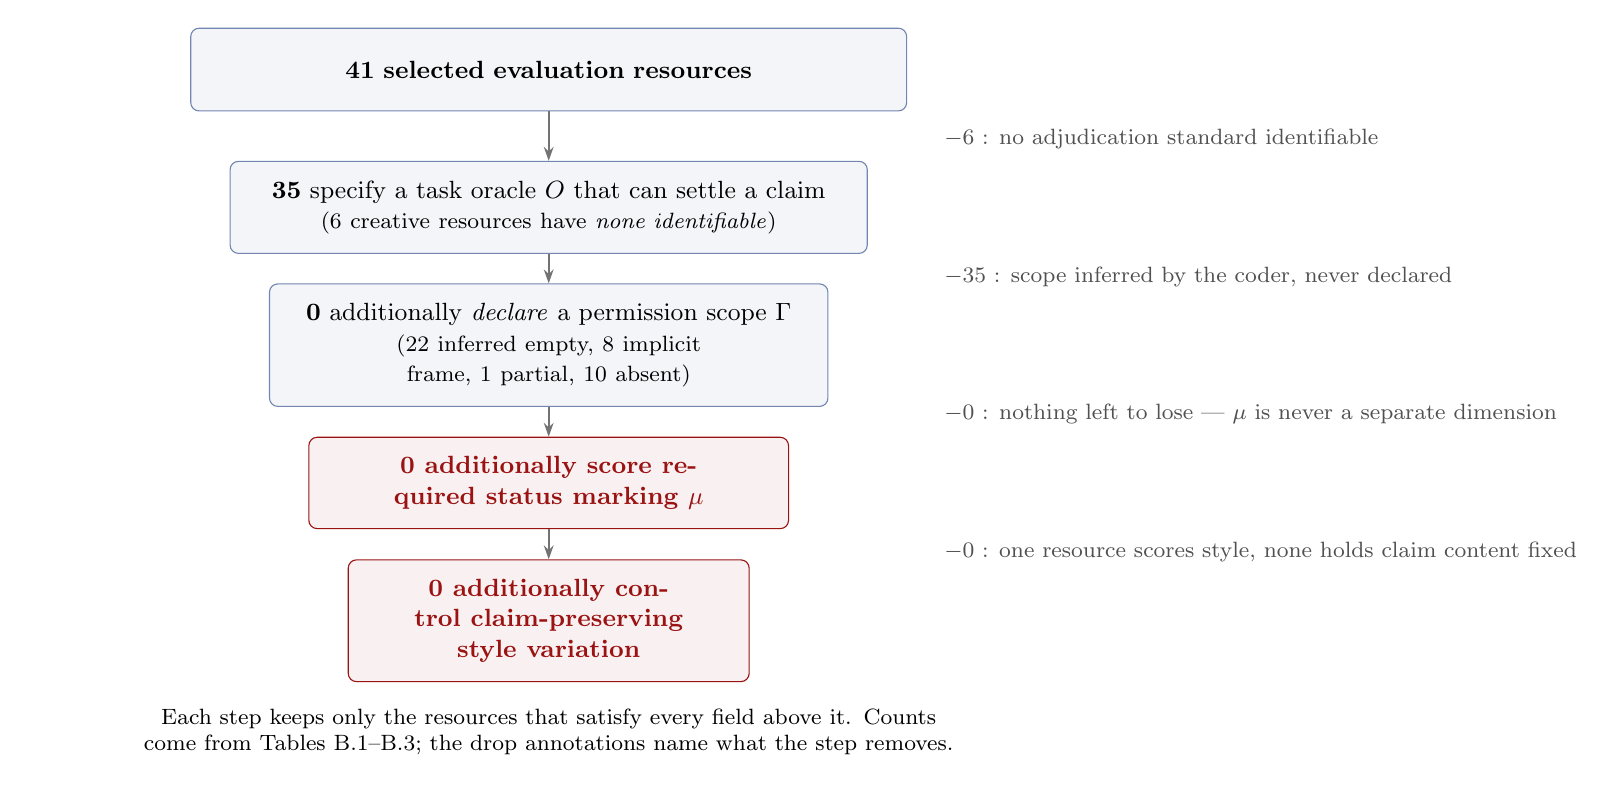
\begin{tikzpicture}[x=1cm,y=1cm,font=\small,
   fstep/.style={rectangle,rounded corners=3pt,draw=clrB!60,fill=clrB!5,
     minimum height=1.05cm,align=center,inner sep=7pt,font=\small},
   dead/.style={rectangle,rounded corners=3pt,draw=clrH,fill=clrH!6,text=clrH,
     minimum height=1.05cm,align=center,inner sep=7pt,font=\small\bfseries},
   drop/.style={font=\footnotesize,text=clrG,anchor=west},
   ar/.style={-{Stealth[length=5pt,width=3.5pt]},thick,draw=black!55}]

  \node[fstep,text width=8.6cm] (s0) at (0,0)
    {\textbf{41 selected evaluation resources}};
  \node[fstep,text width=7.6cm] (s1) at (0,-1.75)
    {\textbf{35} specify a task oracle $O$ that can settle a claim\\
     \footnotesize{(6 creative resources have \emph{none identifiable})}};
  \node[fstep,text width=6.6cm] (s2) at (0,-3.50)
    {\textbf{0} additionally \emph{declare} a permission scope $\Gamma$\\
     \footnotesize{(22 inferred empty, 8 implicit frame, 1 partial, 10 absent)}};
  \node[dead,text width=5.6cm] (s3) at (0,-5.25)
    {\textbf{0} additionally score required status marking $\mu$};
  \node[dead,text width=4.6cm] (s4) at (0,-7.00)
    {\textbf{0} additionally control claim-preserving style variation};

  \draw[ar] (s0) -- (s1); \draw[ar] (s1) -- (s2);
  \draw[ar] (s2) -- (s3); \draw[ar] (s3) -- (s4);

  \node[drop] at (4.9,-0.88) {$-6$ : no adjudication standard identifiable};
  \node[drop] at (4.9,-2.63) {$-35$ : scope inferred by the coder, never declared};
  \node[drop] at (4.9,-4.38) {$-0$ : nothing left to lose --- $\mu$ is never a separate dimension};
  \node[drop] at (4.9,-6.13) {$-0$ : one resource scores style, none holds claim content fixed};

  \node[anchor=north,align=center,font=\footnotesize,text width=13cm] at (0,-8.0)
    {Each step keeps only the resources that satisfy every field above it.
     Counts come from Tables B.1--B.3; the drop annotations name what the step removes.};
\end{tikzpicture}
\end{center}

\vspace{2pt}
\noindent\textbf{Pourquoi elle fonctionne.} C'est la seule des trois qui raconte le r\'esultat comme une
\emph{s\'equence} : le lecteur voit o\`u la litt\'erature s'arr\^ete, et l'\'ecart entre «~l'oracle est presque
toujours l\`a ~» et «~la port\'ee n'est jamais d\'eclar\'ee ~» devient l'information centrale.

\medskip
\noindent\textbf{R\'eserve honn\^ete.} La lecture cumul\'ee peut sugg\'erer une hi\'erarchie de difficult\'e
($O$ facile, $\Gamma$ dur, $\mu$ plus dur) que les donn\'ees ne d\'emontrent pas : l'ordre des \'etapes est
celui du contrat, pas un ordre mesur\'e. Si cette figure est retenue, la l\'egende doit le dire en une phrase.
C'est la raison pour laquelle la Proposition~A reste recommand\'ee.

\clearpage

\section*{Comparaison et recommandation}

\noindent
\begin{tabular}{@{}p{2.4cm}p{4.1cm}p{4.1cm}p{4.1cm}p{4.1cm}@{}}
\toprule
& \textbf{Figure 3 actuelle} & \textbf{A --- matrice par profil} & \textbf{B --- grille par ressource} & \textbf{C --- entonnoir}\\
\midrule
Message en $<$20\,s
& la case en haut \`a gauche est vide
& deux colonnes sont vides
& deux colonnes sont vides, sur 41 items
& la litt\'erature s'arr\^ete \`a l'oracle\\
\addlinespace
R\'esultat principal visible ?
& \textbf{non} --- affirm\'e en l\'egende
& \textbf{oui}
& \textbf{oui}
& \textbf{oui}\\
\addlinespace
Avertissements requis
& 4 phrases + \emph{Reading guide} 6 lignes
& aucun
& aucun
& 1 phrase (ordre non mesur\'e)\\
\addlinespace
Place du style
& un axe entier sur deux
& 1 colonne sur 4
& 1 bloc sur 4
& derni\`ere \'etape\\
\addlinespace
Tra\c cabilit\'e vers B.1--B.3
& num\'eros entre crochets
& via la l\'egende
& \textbf{marque par ressource}
& via les compteurs\\
\addlinespace
Encombrement
& pleine largeur
& \textbf{demi-page, 1 colonne}
& pleine largeur, paysage
& demi-page\\
\bottomrule
\end{tabular}

\vspace{10pt}
\noindent\textbf{Recommandation : Proposition A}, avec la Proposition~B en annexe si un relecteur demande
le d\'etail ressource par ressource. A supprime les quatre avertissements de la l\'egende actuelle, rend le
r\'esultat principal visible, et ram\`ene le style-marking au rang qu'il occupe dans l'argument.

\vspace{8pt}
\noindent\textbf{Point \`a trancher avant int\'egration.} Les propositions A et B distinguent
\yes\ (\emph{separately represented}) de \hf\ (\emph{inferred, implicit or partial}). Cette distinction
n'existe pas telle quelle dans le codage actuel, qui utilise \emph{inferred empty}, \emph{implicit frame},
\emph{partial}, \emph{not separately represented}. Le regroupement propos\'e ici est le suivant, et doit
\^etre valid\'e ou corrig\'e avant toute int\'egration dans le manuscrit :

\vspace{4pt}
\noindent
\begin{tabular}{@{}ll@{}}
\toprule
\textbf{Code du mapping} & \textbf{Regroupement propos\'e}\\
\midrule
$O$ : tout type nomm\'e (source document, gold labels, environment state, \dots) & \yes\\
$O$ : mixed or task-dependent & \hf\\
$O$ : none identifiable & \no\\
$\Gamma$ : inferred empty ; implicit frame ; partial & \hf\ (jamais \yes)\\
$\Gamma$ : not separately represented & \no\\
$\mu$ : not scored ; not separated & \no\ (aucune valeur positive dans le mapping)\\
style : scored, not claim-controlled & \hf\\
style : not controlled ; not controlled or not applicable & \no\\
\bottomrule
\end{tabular}

\end{document}
